\section{Problem Formulation} 
 
Given a subset of data and attributes to be studied, the goal for {\tt VizInNuce} is to  identify the most interesting and informative visualizations summarizing patterns or trends. There are two major challenges in achieving this goal; (i) scale: evaluating a large number of candidate visualizations in lattice while responding within interactive time scales, and (ii) utility: identifying appropriate metrics for assessing interestingness and informativeness of visualizations. For now, we focus on the latter. We first describe two conceptual visualization lattices, and then describe the .

 
 
 
\subsection{Preliminaries} 
A dataset $D$ consists of a set of dimension attributes $A$, and a set of measure attributes $M$. We define a metric family $z$ as the result of a SQL query using a group of dimension attributes $A_z \subseteq A$, a single measure attribute $m_z \in M$, and an aggregate function $f_z$ as follows: {\tt SELECT $A_z$ AS $metric\_id, f(m_z)$ AS $metric\_value$ FROM $D$ GROUP BY $A_z$}. The result of this query can be presented using a table with two columns, where the first column accommodates the metrics within the metric family, and the second column accommodates the values corresponding to these metrics. This two column table can be visualized with a bar chart, where each metric is visualized using a separate bar. 
\newline
\newline
Notice that the aforementioned query does not have a {\tt WHERE} clause. If we include a {\tt WHERE} clause in this query incorporating constraints on the remaining dimension attributes $A_z^\prime = A - A_z$, we shall get different instances of $z$ corresponding to different data subsets defined by the constraints. These different instances of $z$ can be visualized with separate bar charts that present the same metric family for different data subsets. 

\subsection{Data Subset Lattice}
A data subset can be contained within another data subset. Specifically, given a data subset defined by a set of constraints on dimension attributes, adding one or more new constraints in the set will generate a new data subset that is contained within the former subset. We specify a data subset as the \emph{parent} of another data subset if the latter is defined by a set of constraints that includes one additional constraint along with the ones that define the former subset. Notice that, as per our definition, a data subset can have multiple parent subsets.
 \newline
 \newline
We extend the idea of parent data subset to introduce the concept of parent visualization. Let $V_s(z)$ represent the set of visualizations that visualize a metric family $z$ for different data subsets. Given a visualization $v_i \in V_s(z)$ (corresponding to a particular data subset), parent of $v_i$, $v_i^j \in V_s(z)$ is a visualization that corresponds to a parent data subset of the former. Analogous to a data subset, a visualization $v_i \in V_s(z)$ can have multiple parents. 

\begin{figure*}[bht]
\label{example}
\centering
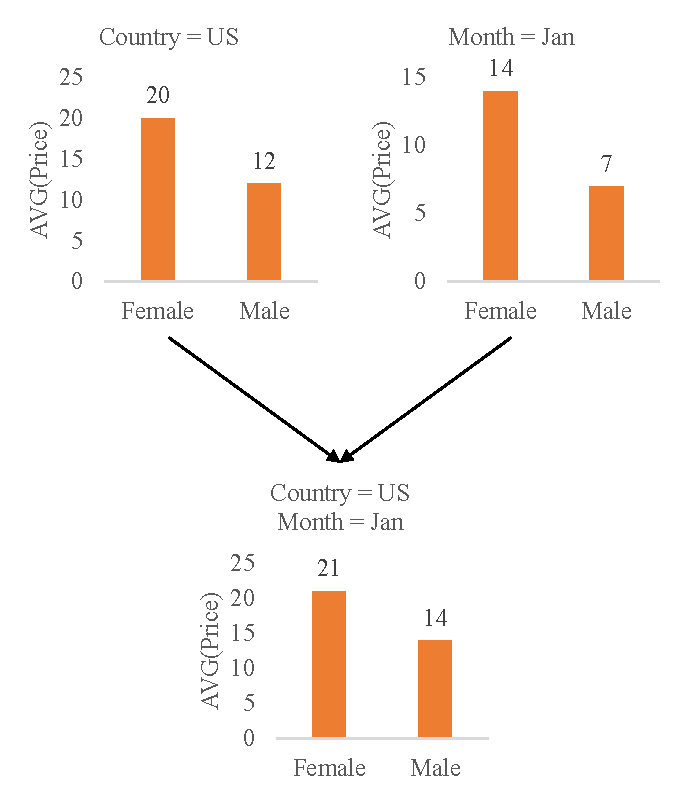
\includegraphics[scale=0.75]{SubsetRelation.pdf}
\caption{Parent Child Relationship in Data Subset Lattice}
\end{figure*}
 



\subsection{Dimension Combination Lattice}
Given a combination of dimension attributes, inducing one or more new dimensions in the combination will generate a new combination. We specify a dimension combination as the \emph{parent} of another dimension combination if the latter is defined by a set of dimensions that includes one additional dimension along with the ones that define the former combination. Notice that, as per our definition, a dimension combination can have multiple parent combinations.
 \newline
 \newline
Let $V_c(Z)$ represent the set of visualizations that visualize the different metric families with same measure of interest and same data subset. We extend the idea of parent dimension combination to introduce the concept of parent visualization. Specifically, given a visualization $v_i \in V_c(Z)$ (corresponding to a particular dimension combination), parent of $v_i$, $v_i^j \in V_c(Z)$ is a visualization that corresponds to a parent dimension combination of the former. Analogous to a dimension combination, a visualization $v_i \in V_c(Z)$ can have multiple parents. 

\begin{figure*}[bht]
\label{example}
\centering
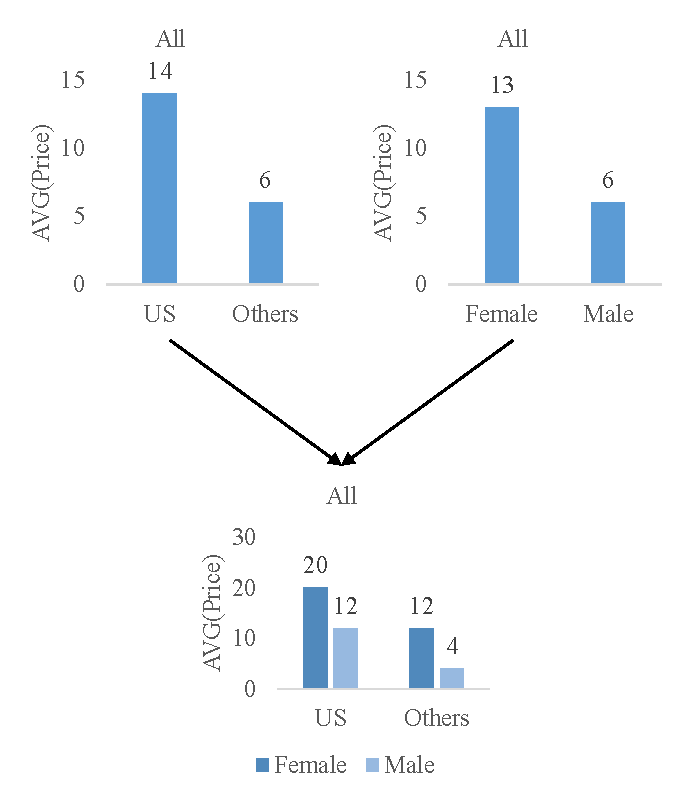
\includegraphics[scale=0.75]{DimensionRelation.pdf}
\caption{Parent Child Relationship in Dimension Combination Lattice}
\end{figure*}
 


\section{Parent Child Relationship Model} 
We observe that, while exploring a dataset, users first look at the top level visualizations before looking at the next level. Further, the knowledge learnt from the top level visualizations set up user expectation for the next level. Based on these two observations, we quantify the parent-child relationship mentioned above.  
  
\subsection{User Expectation Model}
We formulate user expectation ($\hat{v_i}$) corresponding to a visualization $v_i$, based on its parents, $v_i^1, \ldots, v_i^\lambda$. 
  
$$\hat{v_i} = g(v_i^1, \ldots, v_i^\lambda)$$

Here, the function $g()$ takes the parents of $v_i$ as argument and returns user expectation $\hat{v_i}$.
\newline
\newline
We assert that the parents of $v_i$ do not contribute equally in setting up user expectation $\hat{v_i}$. We care about the $p$ parents that contribute most in setting up $\hat{v_i}$. We call these $p$ parents the \emph{true parents} of $v_i$ and represent them as $[v_i^*, p]$. 
  
$$[v_i^*,p] = \underset{v_i^j}{\operatorname{arg\,\,\,max\_p}}\ d(v_i,v_i^j)$$
  %better expressed as top_p_v_i^j??
Here, the function $d()$ takes $v_i$ and its parent $v_i^j$ as argument and returns the contribution of $v_i^j$ in setting up $\hat{v_i}$. 
  
  
  
  % The goal of our problem is as follows: given a metric family $F_\theta$, identify $k$ connected bar charts from $V$, informative yet surprising  to build a dashboard. \newline
  \newline
  
  
  \iffalse
  
  \subsection{User Expectation Graph}
  We construct a user expectation graph $G(V, E, W)$, where vertex set $V = \{v_1, v_2, ..., v_n\}$ represents the bar charts that visualize metric family $F_\theta$ for different subpopulations, edge set $E$ captures the true parent-child relationship between visualizations, and $W$ captures the contribution of true parent in setting up user expectation for child visualization. 
  
$$
     w_{xy} = 
     \begin{cases} 
      d(v_x,v_y), & v_y\in [v_x^*,p] \\
      0, & \mathrm{otherwise}
    \end{cases}
$$

 We formulate our dashboard building problem as follows: given user expectation graph $G(V, E, W)$, the root vertex $v_R \in V$, and an integer $k$, find a subset $V^\prime \subseteq V$ of $k$ vertices such that $v_R \in V^\prime$, the subgraph induced by $V^\prime$ is connected and has maximum total edge weight.
 \subsection{Dashboard Properties}

%   There are alternative ---- that is not considered in our model:  

 \begin{figure}[ht!]
\centering
\includegraphics[width=0.5\linewidth]{plots/ExpectationExample.pdf}
\label{expectation_example}
\caption{Consider a example dataset with several dimension attributes such as \textit{gender}, \textit{state}, etc., and a single measure attribute \textit{population}. A metric}
\end{figure}

\fi

%%%%%%%%%%%%%%%%%%%%%%%%%%%%%%%%%%%%%%%%%%%%%%%%%%%%%%%%%%%%%%%%%%%%%%%%%%%%%%
\section{System Design}
In this report, we discuss the system design choices for our dashboard construction problem. 

\subsection{Dashboard Interface Design}
Dashboard interface design is one of the key design choices in dashboard construction problem. The design of dashboard interface and users' interaction with the interface critically affect the overall system architecture. We particularly focus on the static/dynamic nature of dashboard interface.
\newline
\newline
\textbf{Static Dashboard:} For the static version of dashboard construction problem, our goal is to find the set of k visualizations that maximize our proposed objective function, in a single shot. For this problem, user interaction is limited to the initial selection of sub-population and dimension variables of interest. This static problem has several pros and cons that we list below.

\begin{itemize}
\item Pros: In the static problem, users can specify the amount of time that they are willing to wait. The benefit is that since this does not require user-in-the-loop, a user can specify an arbitrarily long wait-time, e.g., several days, to generate the result. The user can check the result at the end of the specified wait-time. If the specified wait-time is small, the system can generate approximate \emph{good-enough} result.  

\item Cons: Since this problem does not involve user-in-the-loop, the user can not filter or guide the system towards specific attributes/subpopulations that he/she would be interested in, so while the user expectation model updates based on the visualizations that the users have seen along the path, the prior of the expectation model at the start is generic for all users. This yields interesting visualization for analysts to explore previously unseen datasets in a cold-start manner, but the system quickly looses its usefulness as the users learn more about the dataset and have no way to specifying these learned insights to the system.
\end{itemize}
\newline
\newline
\textbf{Dynamic Dashboard:}
 After data loading, the user begins exploring the dashboard in a top-down manner, starting at the root and drilling down.  For each node visited, the user is shown all available child nodes based on the current visualization, the node color indicates how likely would this subpopulation be a promising child to visit. The user has the option to visit the nodes following the system's recommendation or he could chose to view another subpopulation of that he deems interesting.
 
 \begin{figure}[ht!]
\includegraphics[scale=0.3]{MixedInitiativeFig.pdf}
\caption{As an example usage scenario, the user is currently viewing visualization V2, he sees the subpopulation recommendation at the next level, V4 is the most promising child to explore (darkest hue of blue). At the current stage, the user is not allowed to explore any of the greyed out visualizations (unconnected parents or children).}

\end{figure}
 \begin{itemize}
 \item Pros: Mixed initiative approach means that users has input at every step of the exploration regarding the children visualizations that they would like to explore. Compare to direct manipulation of viewing all possible bar charts, the mixed initiative exploration should be more tractable since the pruning done by the system and recommendations done to create the DAG significantly limits the number of bar charts that the users could end up seeing. This would also be more interpretable because the interaction enforces that the visualization explored must be connected through the parent-child relationship. The analyst is able to employ the familiar analogy of drill-down and roll-up to explore the DAG.
 % are we allowing roll-ups to explore other parents? 
 \item Cons: The user's selection of a subpopulation means that we must show that visualization in an online manner, which means we lose out on a lot of the precomputation that we could do if we had known the attributes of interest beforehand (based on data-driven measures, level and subpopulation limit). One way around this is to still apply these constraints specified in the materialization phase and limit the amount of possible child nodes that the analyst could chose from. (i.e. chose between drilling down along v1 or v3 versus chosing between v1,v2,v3,v4,v5 at that level)
 \end{itemize}




\section*{Offline Phase}
\begin{enumerate}
\item  Offline phase: The analyst loads in a dataset of interest and uses the selection tools in the interface to make the following selections:
\begin{itemize}
\item Choice of Root population. The user has the option to start the exploration from a specific subpopulation of interest (e.g. AB). By default, the root is set as the highest level of aggregation, which is equivalent to the whole population.
\item  The amount of time that he is willing to wait for before the interactive stage. By using a cost model, we can translate this budget into an estimate of amount of cube materialization we are allowed to make in the offline stage. 
\item Constraints on the types of visualizations that analyst would like to see. This can be translated into materialization strategies such as material all cubes that satisfy the iceberg criterion or show me only visualizations at level 3 or above.
\item Measure. The analyst selects the measure variable that they are interested in visualizing, such as population or sales.
\item Metrics. Based on our desiderata, 
  \begin{itemize}
    \item Connectedness: Visualizations in a dashboard should present a connected story, i.e., there should be connections/relationships among the chosen visualizations. This is enforced by traversing the DAG from parent to child nodes.
    \item Informativeness: These connections/relationships should be informative rather than misleading. Informativeness is incorporated in our expectation model by chosing the most informative true parent among the multiple parents.
    \item Surprisingness: We are interested in the informative, yet surprising relationships. Surprisingness is measured by deviation from user expectation.
    \item Subpopulation size: Each visualization should cover a significant population. Surprising relationships appearing in the low levels of data (e.g., 0.1\% of tuples) are not of interest.
  \end{itemize}
The first three criterion listed are essential to our current problem formulation, there are other metrics that could be optionally added in to combine to form our objective functions.
\item Visualization objective. What type of visualization insight is the analyst hoping to get from the analysis? (breadth/depth based?). Understanding the users motivation enable us to tune the tradeoff between the parameters that we use in our objective function, to decide on whether to spend our budget on exploring new nodes with different sets of parents or drilling down along the same child visualizations.
\end{itemize}

\end{enumerate}
% Aditya comments:
% - description of user interface
% - user tuning tradeoff between metrics and parameter (knob to tune) vi
%	- breadth and depth based 
% - exploring multiple dimensions , measures , going down multiple measures, (e..g profits and sales, portions that these are not correlated, correlated would be interesting) How does multiple variable relationship change this problem, or is this jsut a matter of tracking multiple measure values? (separate objective?)
% can brushing and linking tools be used for visual summarization? 
 
    